%
\chapter{The pseudo-spectral method} 
\label{chap_pseudspec}
%
The idea behind the pseudo-spectral method is first to transform
the evolution equations to Fourier (spectral) space, i.e.\ in our
example to use the eigenfunctions of the Laplacian as basis of the
space of all solutions and to project the full equations onto this basis,
see e.g.\ \cite{canutoetal1988}. Second to calculate products of functions
(non-linear terms) in the physical space and transform them back
to Fourier space to reduce the number of multiplications necessary,
which otherwise makes the spectral method computationally prohibitively
expensive for problems with a large numbers of Fourier modes. This idea
goes back to \cite{kreissandoliger1972}. More details on the
pseudospectral method can be found, e.g.\ in \cite{orszag1972}
and \cite{fornberg1987}.
%
\section{The discrete Fourier transform}
\label{sec_discretefourier}
%
Starting point for the set of basis functions are the Fourier modes 
$F(k_{x},k_{y} \ | \ x,y)$ which are the eigenmodes of the Laplacian 
on the fluid domain considered (short notation 
$F(\mathbf{k} \ | \ \mathbf{x})$ with 
$\mathbf{k} = (k_{x},k_{y})$ and $\mathbf{x} = (x,y)$).  
We start with a doubly periodic fluid domain (default in CAT). 
In this case the eigenmodes of the Laplacian are given by
\begin{equation} \label{eq_defFkxky}
  F(\mathbf{k} \ | \ \mathbf{x}) 
   = 
 \exp \left[ i  \left(k_{x} x + k_{y} y \right) \right]
   = 
 \exp \left[ i k_{x} x \right] \ 
 \exp \left[ i k_{y} y \right],
\end{equation}
and satisfy the eigenvalue equation
\begin{equation} \label{eq_eigFkxky}
 \Delta \ F(\mathbf{k} \ | \ \mathbf{x})
   =
  - \left( k_{x}^{2} + k_{y}^{2} \right) \ 
    F(\mathbf{k} \ | \ \mathbf{x}),
\end{equation}
with $k_{x} = n \ 2 \pi/X$ and $k_{y} = m \ 2 \pi/Y$ for 
$n,m \in [0,\pm 1, \pm 2,\ \dots \ ]$. As can be seen form equation 
(\ref{eq_defFkxky}) the eigenmodes of the Laplacian on the 
two-dimensional fluid domain 
$F(\mathbf{k} \ | \ \mathbf{x}) = F(k_{x} \ | \ x) \ F(k_{y} \ | \ y)$
can be separated into a product of the eigenmodes of the 
1-dimensional Laplacian. For more general domains
as circular discs, annuli or the surface of spheres as well as 
for more general boundary conditions, i.e. for fluid domains with walls 
one has to choose other systems of basis functions, 
see e.g.\ \cite{canutoetal1988}.

Taking $L_{x} = X/2 \pi$ and $L_{y} = Y/ 2 \pi$ in $x$ and $y$-direction 
as horizontal length scales and introducing the non-dimensional variables
$\bar{x} = x/L_{x}$, $\bar{y} = y/L_{y}$, $\bar{k}_{x} = k_{x} L_{x}$ 
and $\bar{k}_{y} = k_{y} L_{y}$ the non-dimensional eigenvalue equation
\begin{equation} \label{eq_ndeigFkxkyLxLy}
 \left[ 
  \frac{\partial^{2}}{\partial \bar{x}^{2}} 
   +
  \frac{\partial^{2}}{r^{2} \partial \bar{y}^{2}} 
 \right] \ 
  F(\mathbf{\bar{k}} \ | \ \mathbf{\bar{x}})
   = 
  - \left( \bar{k}_{x}^{2} + \frac{\bar{k}_{y}^{2}}{r^{2}} \right)
  F(\mathbf{\bar{k}} \ | \ \mathbf{\bar{x}}),
\end{equation}
with the aspect ratio of the fluid domain $r = L_{y}/L_{y} = Y/X$,
the wave number vector $\mathbf{\bar{k}} = (\bar{k}_{x},\bar{k}_{y})$, 
where $\bar{k}_{x} = \bar{k}_{y} = 0, \pm 1, \pm 2, \ \dots \ $ and the
coordinate vector $\mathbf{\bar{x}} = (\bar{x},\bar{y})$, where 
$\bar{x},\bar{y} \in [0 \ \ 2\pi]$.
Such an approach leads to a rescaled Laplacian and is appropriate 
in particular for physical problems with a strong horizontal 
anisotropy.

Introducing a single horizontal length scale as for example 
$L = L_{x} = X/2 \pi$ instead we get the non-dimensional variables 
$\bar{x} = x/L$, $\bar{y} = y/L$, $\bar{k}_{x} = k_{x} L = n$ and 
$\bar{k}_{y}/r = k_{y} L/r = m/r$. The non-dimensional eigenvalue 
equation now reads
\begin{equation} \label{eq_ndeigFkxkyL}
 \left[ 
  \frac{\partial^{2}}{\partial \bar{x}^{2}} 
   +
  \frac{\partial^{2}}{\partial \bar{y}^{2}} 
 \right] \ 
  F(\mathbf{\bar{k}} \ | \ \mathbf{\bar{x}})
   = 
  - \left( \bar{k}_{x}^{2} + \frac{\bar{k}_{y}^{2}}{r^{2}} \right)
  F(\mathbf{\bar{k}} \ | \ \mathbf{\bar{x}}),
\end{equation}
with the aspect ratio of the fluid domain $r$ defined above, 
the wave number vector $\mathbf{\bar{k}} = (\bar{k}_{x},\bar{k}_{y}/r)$, 
where $\bar{k}_{x} = \bar{k}_{y} = 0, \pm 1, \pm 2, \ \dots \ $ and
the coordinate vector $\mathbf{\bar{x}} = (\bar{x},\bar{y})$, where
$\bar{x} \in [0 \ 2 \pi]$ and $\bar{y} \in [0 \ r 2 \pi]$. 
In CAT we use a single horizontal length scale 
keeping in mind that this choice is not optimal for problems 
with a strong horizontal anisotropy. In the special case of a square domain 
(default case in CAT) we have $r = 1$.
From now on we use, if not otherwise stated, the non-dimensional form and 
omit overbars. 

Using the Fourier modes $F(\mathbf{k} \ | \ \mathbf{x})$ we can expand all 
fields $g(x,y,t)$ on the fluid domain into a Fourier series
\begin{equation} \label{eq_fourierser}
  g(x,y,t) 
   =  
  \sum_{k_{x} = -\infty}^{\infty} \ \sum_{k_{y} = -\infty}^{\infty} \ 
   \hat{g}(k_{x},k_{y},t) \ 
   \exp
   \left[ 
     i \left(k_{x} x + \frac{k_{y}}{r} y \right)
   \right],
\end{equation}
where $\hat{g}(k_{x},k_{y},t)$ are the Fourier coefficients of 
$g(x,y,t)$ which live on the space of wave numbers $(k_{x},k_{y})$.
Since $g(x,y,t)$ are real fields, the Fourier modes $\hat{g}(k_{x},k_{y},t)$
have the symmetry property that
\begin{equation} \label{eq_symfourier}
  \hat{g}(-k_{x},-k_{y},t)  = \hat{g}^{\ast}(k_{x},k_{y},t),
\end{equation}
where $g^{\ast}$ is the complex conjugate of $g$. The Fourier
coefficients $\hat{g}(k_{x},k_{y},t)$ are obtained by the integral
\begin{equation} \label{eq_fourierintndim}
  \hat{g}(k_{x},k_{y},t)
   = 
  \frac{1}{r} \frac{1}{4 \pi^{2}} 
   \int_{0}^{2 \pi} \int_{0}^{r 2 \pi}
   \exp  
   \left[ 
    -i \left(k_{x} x + \frac{k_{y}}{r} y \right)
   \right] \
   g(x,y,t) \ 
dx dy.
\end{equation}
This continous finite Fourier integral is derived from the
dimensional integral 
\begin{equation} \label{eq_fourierint}
  \hat{g}(k_{x},k_{y},t)
   =
  \frac{1}{XY} \int_{0}^{X} \int_{0}^{Y}
   \exp
   \left[
    -i \left(k_{x} x + k_{y} y \right)
   \right] \
   g(x,y,t) \
dx dy,
\end{equation}
where $x$,$y$,$k_{x}$ and $k_{y}$ are the dimensional variables.

To use the Fourier transform in numerical schemes to solve the evolution
equation of fluids we have to approximate the continous finite Fourier integral
(\ref{eq_fourierintndim}) and the infinite Fourier series
(\ref{eq_fourierser}).

We start by discretizing the physical space into $N$ grid points in
$x$-direction and $M$ grid points in $y$-direction. On the discretized
grid of the physical space the continuous finite Fourier integral
(\ref{eq_fourierintndim}) reduces to the double sum
\begin{equation} \label{eq_fourierintprox}
   \hat{g}(k_{x},k_{y},t)
    = 
   \frac{1}{N M} 
   \sum_{n = 0}^{N-1} \sum_{m=0}^{M-1} \
    \exp 
     \left[-i    
      \left(
       k_{x} x_{n} + \frac{k_{y}}{r} y_{m}
      \right)
     \right]
     g(x_{n},y_{m},t),
\end{equation}
where we use the approximations $dx = \Delta x =2\pi/N$, 
$dy = \Delta y = r 2\pi/M $, $x_{n} = n \ \Delta x$ 
and $y_{m} = m \ \Delta y$ with $n \in [0,1,\ \dots \ ,N-1]$ and
$m \in [0,1,\ \dots \,M-1]$. The aspect ratio of the grid cell 
is given by $\Delta x/\Delta y = M/N \ 1/r$. For $r = M/N$ 
the grid cells are squares (default in CAT $M=N$ and $r=1$).
 
Next we truncate the infinite Fourier series (\ref{eq_fourierser}) 
at wave numbers such that all modes with a higher spatial frequency 
(wave mumber) than the grid in physical space are omitted otherwise
we would have an oversampling. The result is the finite sum
\begin{equation} \label{eq_fouriersertrun}
  g(x_{n},y_{m},t) 
   =  
  \sum_{k_{x} = -\frac{N}{2}+1}^{\frac{N}{2}} \ 
  \sum_{k_{y} = -\frac{M}{2}+1}^{\frac{M}{2}} \
   \exp
   \left[ 
    i \left(k_{x} x_{n} + \frac{k_{y}}{r} y_{m} \right)
   \right] \
   \hat{g}(k_{x},k_{y},t).
\end{equation}
On the discretized grid in the physical space the modes with wave numbers 
$(k_{x},k_{y}) = (-N/2,-M/2)$ and $(k_{x},k_{y}) = (N/2,M/2)$ are 
identical. We omitted the mode $(k_{x},k_{y}) = (-N/2,-M/2)$.

Using the definitions of $x_{n} = 2 \pi \ n/N$ and $y_{m} = r 2 \pi \ m/M$ 
we can write equation (\ref{eq_fourierintprox}) in discretized form as
\begin{equation} \label{eq_fourierintdisc}
  \hat{g}(k_{x},k_{y},t)
   = 
  \frac{1}{NM} 
   \sum_{n = 0}^{N-1}
    \sum_{m = 0}^{M-1}
     \exp 
      \left[
       -i 2 \pi 
        \left( 
         \frac{k_{x} n}{N} + \frac{k_{y} m}{M}
        \right)
      \right]
      \ g(x_{n},y_{m},t)
\end{equation}
and equation (\ref{eq_fouriersertrun}) as
\begin{equation} \label{eq_fourierserdisc}
  g(x_{n},y_{m},t)
   = 
   \sum_{k_{x}= -\frac{N}{2}+1}^{\frac{N}{2}}
    \ 
    \sum_{k_{y}= -\frac{M}{2}+1}^{\frac{M}{2}}
     \exp 
      \left[ 
        i 2 \pi 
        \left( 
         \frac{k_{x} n}{N} + \frac{k_{y} m}{M}
        \right) 
      \right]
    \hat{g}(k_{x},k_{y},t).
\end{equation}
By a shift of the wave numbers $k_{x}$ and $k_{y}$ corresponding to a rotation 
in the complex plane the double sum (\ref{eq_fourierserdisc}) can be written
equivalently in the form
\begin{equation} \label{eq_fourierserdiscshift}
  g(x_{n},y_{m},t)
   = 
   \sum_{k_{x}= 0}^{N-1}
    \ 
    \sum_{k_{y}= 0}^{M-1}
     \exp 
      \left[ 
        i 2 \pi 
        \left( 
         \frac{k_{x} n}{N} + \frac{k_{y} m}{M}
        \right) 
      \right]
    \hat{g}(k_{x},k_{y},t).
\end{equation}
Relation (\ref{eq_fourierintdisc}) defines the discrete $2$-D
forward Fourier transform $\mathcal{F}_{NM}$ and relation 
(\ref{eq_fourierserdiscshift}) the discrete $2$-D inverse Fourier 
transform $\mathcal{F}^{-1}_{MN}$ respectively. One can decompose the 
$2$-D transformations $\mathcal{F}_{NM}$ and $\mathcal{F}^{-1}_{MN}$ 
into two consecutive $1$-D Fourier transformations $\mathcal{F}_{N}$, 
$\mathcal{F}_{M}$ and $\mathcal{F}^{-1}_{M}$, $\mathcal{F}^{-1}_{N}$. 

The forward Fourier transform can be decomposed as follows
\begin{equation} \label{eq_forwardfourier_2D1D}
  \hat{g}(k_{x},k_{y},t) 
    = 
  \frac{1}{N} \sum_{n=0}^{N-1} 
     \exp 
      \left( 
        - i 2 \pi \frac{k_{x} n}{N}
      \right)
  \left[
   \frac{1}{M} \sum_{m=0}^{M-1} 
      \exp 
       \left( 
         - i 2 \pi \frac{k_{y} m}{M}
       \right)
   g(x_{n},y_{m},t) 
  \right]
\end{equation}
or using operators $\hat{g} = \mathcal{F}_{NM} \ g 
= \mathcal{F}_{N} \mathcal{F}_{M} g$, where the operators 
$\mathcal{F}_{N}$ and $\mathcal{F}_{M}$ have the matrix 
representation
\begin{equation} \label{eq_forwardfourier_1D}
  \mathcal{F}_{N} = 
   \frac{1}{N} \ 
   \left(
     exp \left[-i 2 \pi \frac{k_{x} n}{N} \right]
   \right)_{k_{x},n \in [0,N-1]}
   \ \ \mbox{and} \ \ 
  \mathcal{F}_{M} = 
   \frac{1}{M} \ 
   \left(
     exp \left[-i 2 \pi \frac{k_{y} m}{M} \right]
   \right)_{k_{y},m \in [0,M-1]}
\end{equation}
For the inverse Fourier transform we get the decomposition
\begin{equation} \label{eq_inversefourier_2D1D}
  g(x_{n},y_{m},t)
    = 
  \sum_{k_{y}=0}^{M-1}
     \exp
      \left( 
          i 2 \pi \frac{k_{y} m}{M}
      \right)
  \left[
   \sum_{k_{x}=0}^{N-1} 
      \exp 
       \left( 
          i 2 \pi \frac{k_{x} n}{N}
       \right)
   \hat{g}(k_{x},k_{y},t)
  \right],
\end{equation}
which using operators can be written as 
$g=\mathcal{F}^{-1}_{MN}=\mathcal{F}^{-1}_{M} \mathcal{F}^{-1}_{N} \hat{g}$, 
where the operators $\mathcal{F}^{-1}_{N}$ and $\mathcal{F}^{-1}_{M}$ 
have the matrix representation
\begin{equation} \label{eq_inversefourier_1D}
  \mathcal{F}^{-1}_{N} = 
   \left(
     exp \left[i 2 \pi \frac{k_{x} n}{N} \right]
   \right)_{n,k_{x} \in [0,N-1]}
   \ \ \mbox{and} \ \ 
  \mathcal{F}^{-1}_{M} = 
   \left(
     exp \left[i 2 \pi \frac{k_{y} m}{M} \right]
   \right)_{m,k_{y} \in [0,M-1]}.
\end{equation}
Using as basic unit the exponent $\omega = \exp \left[-i 2 \pi/N \right]$
we can represent the one-dimensional discrete forward Fourier transform
$\mathcal{F}_{N}$ for a vector of length $N$ as
\begin{equation} \label{eq_forwardfourier_1D_matrix}
 \mathcal{F}_{N}
  =
 \frac{1}{N} \ 
 \left(
  \begin{array}{ccccc}
    1 &    1         &     1           & \dots & 1
   \\
    1 & \omega       & \omega^{2}      & \dots & \omega^{N-1}
   \\
    . &    .         &     .           &       & . 
   \\
    . &    .         &     .           &       & .
   \\
    . &    .         &     .           &       & .
   \\
    1 & \omega^{N-1} & \omega^{2(N-1)} & \dots & \omega^{(N-1)^{2}}
  \end{array}
 \right). 
\end{equation}
The representation of the Fourier matrices for small $N$ are the building 
blocks of the fast Fourier transform introduced in section (\ref{sec_fft}).   
For $N = 2$, $N = 3$ and $N = 4$ we get
\begin{equation} \label{eq_F2F3F4}
 \mathcal{F}_{2}
  =
 \frac{1}{2}
 \left(
  \begin{array}{cr}
     1  &  1 
        \\
     1  &  -1 
  \end{array}
 \right),
 \ \ 
 \mathcal{F}_{3}
  =
 \frac{1}{3}
 \left(
  \begin{array}{ccc}
     1    &    1         &    1
              \\
     1    & \omega       &  \bar{\omega}
              \\
     1    & \bar{\omega} &  \omega 
  \end{array}
 \right)
\ \ \ \mbox{and} \ \ \ 
 \mathcal{F}_{4}
  =
 \frac{1}{4}
 \left(
  \begin{array}{crrr}
   1   & 1   &  1  &  1
        \\
   1   & -i  & -1  &  i
        \\
   1   & -1  &  1  & -1
        \\
   1   &  i  & -1  & -i 
  \end{array}
 \right),
\end{equation}
with $\omega = -\exp (i \pi/3)=-(\cos(\pi/3)+i \ \sin(\pi/3))$. For $N=8$ 
the representation reads     
\begin{equation} \label{eq_F8}
 \mathcal{F}_{8}
  =
 \frac{1}{8}
 \left(
  \begin{array}{crrrrrrr}
   1 & 1        &  1 &  1       &  1 & 1        &  1 & 1
                                           \\
   1 & \omega   & -i & -i\omega & -1 & -\omega  &  i & i\omega 
                                           \\
   1 & -i       & -1 &  i       &  1 & -i       & -1 & i
                                           \\ 
   1 & -i\omega &  i &  \omega  & -1 & i\omega  & -i & -\omega
                                           \\  
   1 & -1       &  1 & -1       &  1 & -1       &  1 & -1
                                           \\ 
   1 & -\omega  & -i &  i\omega & -1 & \omega   &  i & -i\omega 
                                           \\ 
   1 & i        & -1 & -i       &  1 & i        & -1 & -i 
                                           \\ 
   1 & i\omega  &  i & -\omega  & -1 & -i\omega & -i & \omega 
  \end{array}
 \right),
\end{equation}
with 
$\omega = \exp(-i \pi /4) = \sqrt{0.5} \ (1 - i) = 
 \sqrt{2} \ (1 - i)/2$. 
The inverse Fourier transform $\mathcal{F}^{-1}_{N}$ is given by 
\begin{equation} \label{eq_inversefourier_1D_matrix}
 \mathcal{F}^{-1}_{N}
  =
 \left(
  \begin{array}{ccccc}
    1 &    1         &     1           & \dots & 1
   \\
    1 & \omega       & \omega^{2}      & \dots & \omega^{N-1}
   \\
    . &    .         &     .           &       & . 
   \\
    . &    .         &     .           &       & .
   \\
    . &    .         &     .           &       & .
   \\
    1 & \omega^{N-1} & \omega^{2(N-1)} & \dots & \omega^{(N-1)^{2}}
  \end{array}
 \right), 
\end{equation}
with $\omega = exp \left[i 2 \pi / N   \right]$. The matrix
representation (\ref{eq_inversefourier_1D_matrix}) of the inverse
FFT is related to the matrix representation 
(\ref{eq_forwardfourier_1D_matrix}) of the forward FFT by
omission of the multiplication factor $1/N$ and the
the replacement of $\omega$ by its complex conjugate 
$\bar{\omega}$. Using this rule it is straightforward to derive
the matrix representations of the elementary inverse FFT
operators $\mathcal{F}^{-1}_{2}$, $\mathcal{F}^{-1}_{3}$, 
$\mathcal{F}^{-1}_{4}$ and $\mathcal{F}^{-1}_{8}$.

Making full use of the information hidden in the structure of the 
Fourier matrices (forward and inverse) one can reduce the number 
of multiplications needed to carry out the Fourier transform from 
order {\it O}($N^2$) to order {\it O}($N \log N$), which makes a
big difference for large $N$, see section \ref{sec_fft}.
%
\section{Fast Fourier Transform} 
\label{sec_fft}
%
Keeping the matrix representation the decompostion of the
discrete Fourier operator in order to reduce the number 
of multiplication can down in the case of a factor $2$
decomposition in the following way.
Rearranging the rows of a Fourier matrix $\mathcal{F}_{N}$
by collecting even and odd rows (assuming even $N$) we
can express $\mathcal{F}_N$ in terms of $\mathcal{F}_{N/2}$
and get
\begin{equation}  \label{eq_FNFNr2}
 \mathcal{F}_{N} \ \vec{g}_{N} 
  =
 \left(
  \begin{array}{cr}
   I_{N/2} &  D_{N/2}
           \\
   I_{N/2} & -D_{N/2}
  \end{array}
 \right)
 \left(
  \begin{array}{cr}
   \mathcal{F}_{N/2} &     0
           \\
        0            & \mathcal{F}_{N/2}
  \end{array}
 \right)
 \left(     
  \begin{array}{c}
   \vec{g}_{N/2}^{1}
    \\
   \vec{g}_{N/2}^{2}
  \end{array} 
 \right),
\end{equation} 
where $\vec{g}^{1}_{N/2}$ and $\vec{g}^{2}_{N/2}$ are the odd and even 
components of the vector $\vec{g}_{N}$. Moreover 
$\mathcal{F}_{N/2}$ is the Fourier transform of size $N/2$, 
$I_{N/2}=diag_{N/2}(1,1, \ \dots \ ,1)$ the identity
matrix of size $N/2$ and $D_{N/2}$ the diagonal matrix 
$D_{N/2} =  diag_{N/2}(1,\omega_{N},\ \dots \ , \omega_{N}^{N/2 - 1})$,
with $\omega_{N} = \exp ( -i 2 \pi / N )$. Transforming expression 
(\ref{eq_FNFNr2}) further we can write
\begin{equation}  \label{eq_FNFNr2_01}
 \mathcal{F}_{N} \ \vec{g}_{N}
  =
 \left(
  \begin{array}{cr}
   I_{N/2} &  I_{N/2}
           \\
   I_{N/2} & -I_{N/2}
  \end{array}
 \right)
 \left(
  \begin{array}{cr}
   I_{N/2} &     0
          \\
      0    &   D_{N/2}
  \end{array}
 \right)
 \left(
  \begin{array}{cr}
   \mathcal{F}_{N/2} &     0
           \\
        0            & \mathcal{F}_{N/2}
  \end{array}
 \right)
  \ P_{2,N} \ \vec{g}_{N}
\end{equation} 
where $P_{2,N}$ is a permutation matrix reordering the 
vector components into $2$ blocks (even and odd). Since
the Fourier operators $\mathcal{F}_{N}$ are symmetric we can
write the factor $2$ decomposition also in the form       
\begin{equation} \label{eq_FNFNr2_02} 
 \mathcal{F}_{N} \ \vec{g}_{N}
   = 
 \left[ \mathcal{F}_{2} \otimes I_{N/2} \right] \ 
 \mathcal{D}_{2} \ 
 \left[ I_{2} \otimes \mathcal{F}_{N/2} \right] \
 P_{2,N} \ \vec{g}_{N},
\end{equation}
where the direct matrix products 
$\left[ \mathcal{F}_{2} \otimes I_{N/2} \right]$ and  
$\left[ I_{2} \otimes \mathcal{F}_{N/2} \right]$ 
are defined as the following block 
matrices 
\begin{equation} \label{eq_dirmatprod}
 \left[ \mathcal{F}_{2} \otimes I_{N/2} \right]  
   = 
 \left(
  \begin{array}{cr}
    I_{N/2} & I_{N/2}
                      \\ 
    I_{N/2} & -I_{N/2}
  \end{array}
 \right)
 \ \ \ \mbox{and} \ \ \ 
\left[ I_{2} \otimes \mathcal{F}_{N/2} \right] = \left(\begin{array}{cc} \mathcal{F}_{N/2} &     0 \\ 
     0                & \mathcal{F}_{N/2}
  \end{array}
 \right).
\end{equation}
The diagonal matrix $\mathcal{D}_{2}$ is given by
$diag_{2}(I_{N/2},D_{N/2})$.
Using this decomposition we can reduce the order of the 
Fourier operator by two.  Taking the Fourier operator 
$\mathcal{F}_{4}$ as first example we get 
\begin{equation} \label{eq_exF4twoF2}
\mathcal{F}_{4} \ \vec{g}_{4}
 = 
 \left(
  \begin{array}{crrr}
   1 & 0 & 1 & 0
        \\
   0 & 1 & 0 & 1
        \\
   1 & 0 &-1 & 0
        \\
   0 & 1 & 0 &-1 
  \end{array}
 \right)
 \left(
  \begin{array}{crrr}
   1 & 0 & 0 & 0
        \\
   0 & 1 & 0 & 0
        \\
   0 & 0 & 1 & 0
        \\
   0 & 0 & 0 &-i 
  \end{array}
 \right)
 \left(
  \begin{array}{crrr}
   1 & 1 & 0 & 0
        \\
   1 &-1 & 0 & 0
        \\
   0 & 0 & 1 & 1
        \\
   0 & 0 & 1 &-1 
  \end{array}
 \right)
 \left(
  \begin{array}{crrr}
   1 & 0 & 0 & 0
        \\
   0 & 0 & 1 & 0
        \\
   0 & 1 & 0 & 0
        \\
   0 & 0 & 0 & 1
  \end{array}
 \right) 
  \ \vec{g}_{4} 
\end{equation}
As we see the Fourier operator is decomposed into sparse matrices of 
a very simple form. For matrix entries with a $0$ the multiplication and
summation can be skipped. For entries with $1$, $-1$, $i$ and $-i$ 
multiplication can be skipped. Only signs have to be changed and if needed
real parts have to be shifted to imaginary parts and vice versa. 
It is also possible to reduce the order of Fourier operators by a
factor of $4$. In this case the decomposition reads     
\begin{equation} \label{eq_FNFNr4}
 \mathcal{F}_{N} \ \vec{g}_{N} 
   = 
 \left[
  \mathcal{F}_{4} \otimes I_{N/4}
 \right] \ 
 \mathcal{D}_{4} \
 \left[
  I_{4} \otimes \mathcal{F}_{N/4}
 \right] 
 P_{4,N} \ \vec{g}_{N},
\end{equation}
where 
\begin{eqnarray} \label{eq_FNFNr4def01}
 \left[
  \mathcal{F}_{4} \otimes I_{N/4}
 \right]
 &=&
 \left(
  \begin{array}{rrrr}
   I_{N/4} & I_{N/4} & I_{N/4} & I_{N/4} 
   \\
   I_{N/4} & -iI_{N/4} & -I_{N/4} & iI_{N/4} 
   \\
   I_{N/4} & -I_{N/4} & I_{N/4} & -I_{N/4} 
   \\
   I_{N/4} & iI_{N/4} & -I_{N/4} & -iI_{N/4} 
  \end{array}
 \right) \ 
  \\  
  \\  \label{eq_FNFNr4def02}
 \left[
  I_{4} \otimes \mathcal{F}_{N/4}
 \right]
 &=&
 \left(
  \begin{array}{cccc}
   \mathcal{F}_{N/4} &  0  &   0  &  0
   \\
       0   & \mathcal{F}_{N/4} & 0 & 0
   \\
       0   &   0   & \mathcal{F}_{N/4} & 0
   \\
       0   &   0     &  0  &  \mathcal{F}_{N/4}
  \end{array}
 \right) \ \ \ \mbox{and} \ \ 
  \\  
  \\  \label{eq_FNFNr4def03}
 \mathcal{D}_{4} 
 &=&
 diag_{4} \left(I_{N/4},D_{N/4},D^{2}_{N/4},D^{3}_{N/4} \right).
\end{eqnarray}
The permutation matrix $P_{4,N}$ maps the input vector $\vec{g}_{N}$ to
$\left[ \ \vec{g}^{1}_{N/4},\vec{g}^{2}_{N/4},
\vec{g}^{3}_{N/4},\vec{g}^{4}_{N/4} \ \right]$, a $4$-component vector, with
the $k-th$ components $\vec{g}^{k}_{N/4} = 
\left[ \ k,k+4,k+8, \dots ,k+ (N/4 - 1) \ 4 \  \right]$. Taking $N=8$ as example
and writing $P_{4,8} \ \vec{g}_{8}$ as a $4$-component vector we get
\begin{equation} \label{eq_F8ex01}
 \mathcal{F}_{8} \ \vec{g}_{8}
  = 
 \frac{1}{4}
  \left(
   \begin{array}{rrrr}
    I_{2} & I_{2} & I_{2} & I_{2} 
    \\
    I_{2} & -iI_{2} & -I_{2} & iI_{2} 
    \\
    I_{2} & -I_{2} & I_{2} & -I_{2} 
    \\
    I_{2} & iI_{2} & -I_{2} & -iI_{2}
   \end{array}
  \right) 
  \left(
   \begin{array}{cccc}
    I_{2} &  0    &  0        &  0
    \\
      0   & D_{2} &  0        &  0
    \\
      0   &   0   & D^{2}_{2} &  0
    \\
      0   &   0   &   0       & D^{3}_{2}
   \end{array}
  \right)
  \left(
   \begin{array}{cccc}
    \mathcal{F}_{2} &  0  &   0  &  0
    \\
        0   & \mathcal{F}_{2} & 0 & 0
    \\
        0   &   0   & \mathcal{F}_{2} & 0
    \\
        0   &   0     &  0  &  \mathcal{F}_{2}
   \end{array}
  \right)
  \left(
   \begin{array}{c}
    \vec{g}^{1}_{2}
     \\
    \vec{g}^{2}_{2}
     \\
    \vec{g}^{3}_{2}
     \\
    \vec{g}^{4}_{2}
   \end{array}
  \right),
\end{equation}
with
\begin{equation} \label{eq_F8ex02}
 D_{2} 
  = 
 \left(
  \begin{array}{cc}
    1 & 0
    \\
    0 & \omega
  \end{array}
 \right)
 , \ 
 \vec{g}^{k}_{2} 
  =
 \left(
  \begin{array}{c}
   g_{k}
   \\
   g_{k+4}
  \end{array}
 \right)
 \ \ \mbox{and} \ \
 \omega 
  =
 \sqrt{2} \  \frac{1 - i}{2}.
\end{equation}
Finally the FFT-scheme of CAT includes a factor $8$ decomposition
\begin{equation}  \label{eq_FNFNr8}
 \mathcal{F}_{N} \ \vec{g}_{N} 
   = 
 \left[
  \mathcal{F}_{8} \otimes I_{N/8}
 \right] \ 
  \mathcal{D}_{8} \ 
 \left[
  I_{8} \otimes \mathcal{F}_{N/8}
 \right] 
 P_{8,N} \ \vec{g}_{N},
\end{equation}
with
\begin{equation}  \label{eq_FNFNr8def01}
 \mathcal{D}_{8} =  
 diag_{8} \left(I_{N/8},D_{N/8},D^{2}_{N/8},D^{3}_{N/8}
                D^{4}_{N/8},D^{5}_{N/8},D^{6}_{N/8},D^{7}_{N/8} \right).
\end{equation}
Using the property that the fourier transform is a symmetric operator 
$\mathcal{F}^{T}_{N} = \mathcal{F}_{N}$ the above factorizations can also 
be written equivalently in different forms. For the factor $2$, $4$ and 
$8$ decompositions we get
\begin{eqnarray}  \label{eq_FNFNr2_T}
 \mathcal{F}_{N} \ \vec{g}_{N}
  &=&
 P^{T}_{2,N} \left[I_{2} \otimes \mathcal{F}_{N/2} \right] 
 \mathcal{D}_{2} \ 
 \left[\mathcal{F}_{2} \otimes I_{N/2} \right] \ 
 \vec{g}_{N},
  \\ \label{eq_FNFNr4_T}
 \mathcal{F}_{N} \ \vec{g}_{N}
  &=&
 P^{T}_{4,N} \left[I_{4} \otimes \mathcal{F}_{N/4} \right] 
 \mathcal{D}_{4} \ 
 \left[\mathcal{F}_{4} \otimes I_{N/4} \right] \ 
 \vec{g}_{N}
 \ \ \ \ \mbox{and} \ \
  \\ \label{eq_FNFNr8_T}
 \mathcal{F}_{N} \ \vec{g}_{N}
  &=&
 P^{T}_{8,N} \left[I_{8} \otimes \mathcal{F}_{N/8} \right]
 \mathcal{D}_{8} \ 
 \left[\mathcal{F}_{8} \otimes I_{N/8} \right] \ 
 \vec{g}_{N}.
\end{eqnarray}
The numerical implementation decomposes the original FFT operator 
$\mathcal{F}_{N}$ of order $N$ recursively to a product of operators
which only contain elmentary FFT operators $\mathcal{F}_{N_{k}}$ 
where the orders $N_{k}$ are small prime numbers. In CAT the orders 
of the elementary operators used in the decomposition are 
$N_{k} = 2,4,8$. The inverse FFT can be decomposed in the same way
as the forward FFT 
\begin{eqnarray}  \label{eq_FNFNr2_inverse}
 \mathcal{F}^{-1}_{N} \ \vec{g}_{N}
  &=&
 \left[\mathcal{F}^{-1}_{2} \otimes I_{N/2} \right]
 \mathcal{D}^{-1}_{2} \ 
 \left[I_{2} \otimes \mathcal{F}^{-1}_{N/2} \right] \
 P_{2,N}
 \vec{g}_{N},
  \\ \label{eq_FNFNr4_inverse}
 \mathcal{F}^{-1}_{N} \ \vec{g}_{N}
  &=&
 \left[\mathcal{F}^{-1}_{4} \otimes I_{N/4} \right]
 \mathcal{D}^{-1}_{4} \
 \left[I_{4} \otimes \mathcal{F}^{-1}_{N/4} \right] 
 P_{4,N}
 \vec{g}_{N}
 \ \ \ \ \mbox{and} \ \
  \\ \label{eq_FNFNr8_inverse}
 \mathcal{F}^{-1}_{N} \ \vec{g}_{N}
  &=&
 \left[\mathcal{F}^{-1}_{8} \otimes I_{N/8} \right]
 \mathcal{D}^{-1}_{8} \
 \left[I_{8} \otimes \mathcal{F}^{-1}_{N/8} \right] \
  P_{8,N}
 \vec{g}_{N}.
\end{eqnarray}
Moreover we can again use the symmetry of the inverse FFT 
$\mathcal{F}^{-1}_{N} = \mathcal{F}^{-1 \ T}_{N}$ to get the
equivalent decomposition
\begin{eqnarray}  \label{eq_FNFNr2_Tinverse}
 \mathcal{F}^{-1}_{N} \ \vec{g}_{N}
  &=&
 P^{T}_{2,N}
 \left[I_{2} \otimes \mathcal{F}^{-1}_{N/2} \right]
 \mathcal{D}^{-1}_{2} \ 
 \left[\mathcal{F}^{-1}_{2} \otimes I_{N/2} \right] \ 
 \vec{g}_{N},
  \\ \label{eq_FNFNr4_Tinverse}
 \mathcal{F}^{-1}_{N} \ \vec{g}_{N}
  &=&
 P^{T}_{4,N}
 \left[I_{4} \otimes \mathcal{F}^{-1}_{N/4} \right] 
 \mathcal{D}^{-1}_{4} \ 
 \left[\mathcal{F}^{-1}_{4} \otimes I_{N/4} \right] \ 
 \vec{g}_{N}
 \ \ \ \ \mbox{and} \ \
  \\ \label{eq_FNFNr8_Tinverse}
 \mathcal{F}^{-1}_{N} \ \vec{g}_{N}
  &=&
  P^{T}_{8,N}
 \left[I_{8} \otimes \mathcal{F}^{-1}_{N/8} \right]
 \mathcal{D}^{-1}_{8} \
 \left[\mathcal{F}^{-1}_{8} \otimes I_{N/8} \right] \ 
 \vec{g}_{N}.
\end{eqnarray}
Due to the sparse matrices with the special direct product structure 
it is much more efficient to implement the FFT operator decompositions 
given in euqations 
(\ref{eq_FNFNr2}) to (\ref{eq_FNFNr8}) or (\ref{eq_FNFNr2_T}) to
(\ref{eq_FNFNr8_T}) not as matrix operators but directly as permuations
of memory addresses and hard-coded arithmetic operations.

\vspace{0.5cm}
{\large \bf Text FFT Edilbert?}
%
\section{The grid representation in CAT}
\label{sec_grids}
%
\begin{figure}
   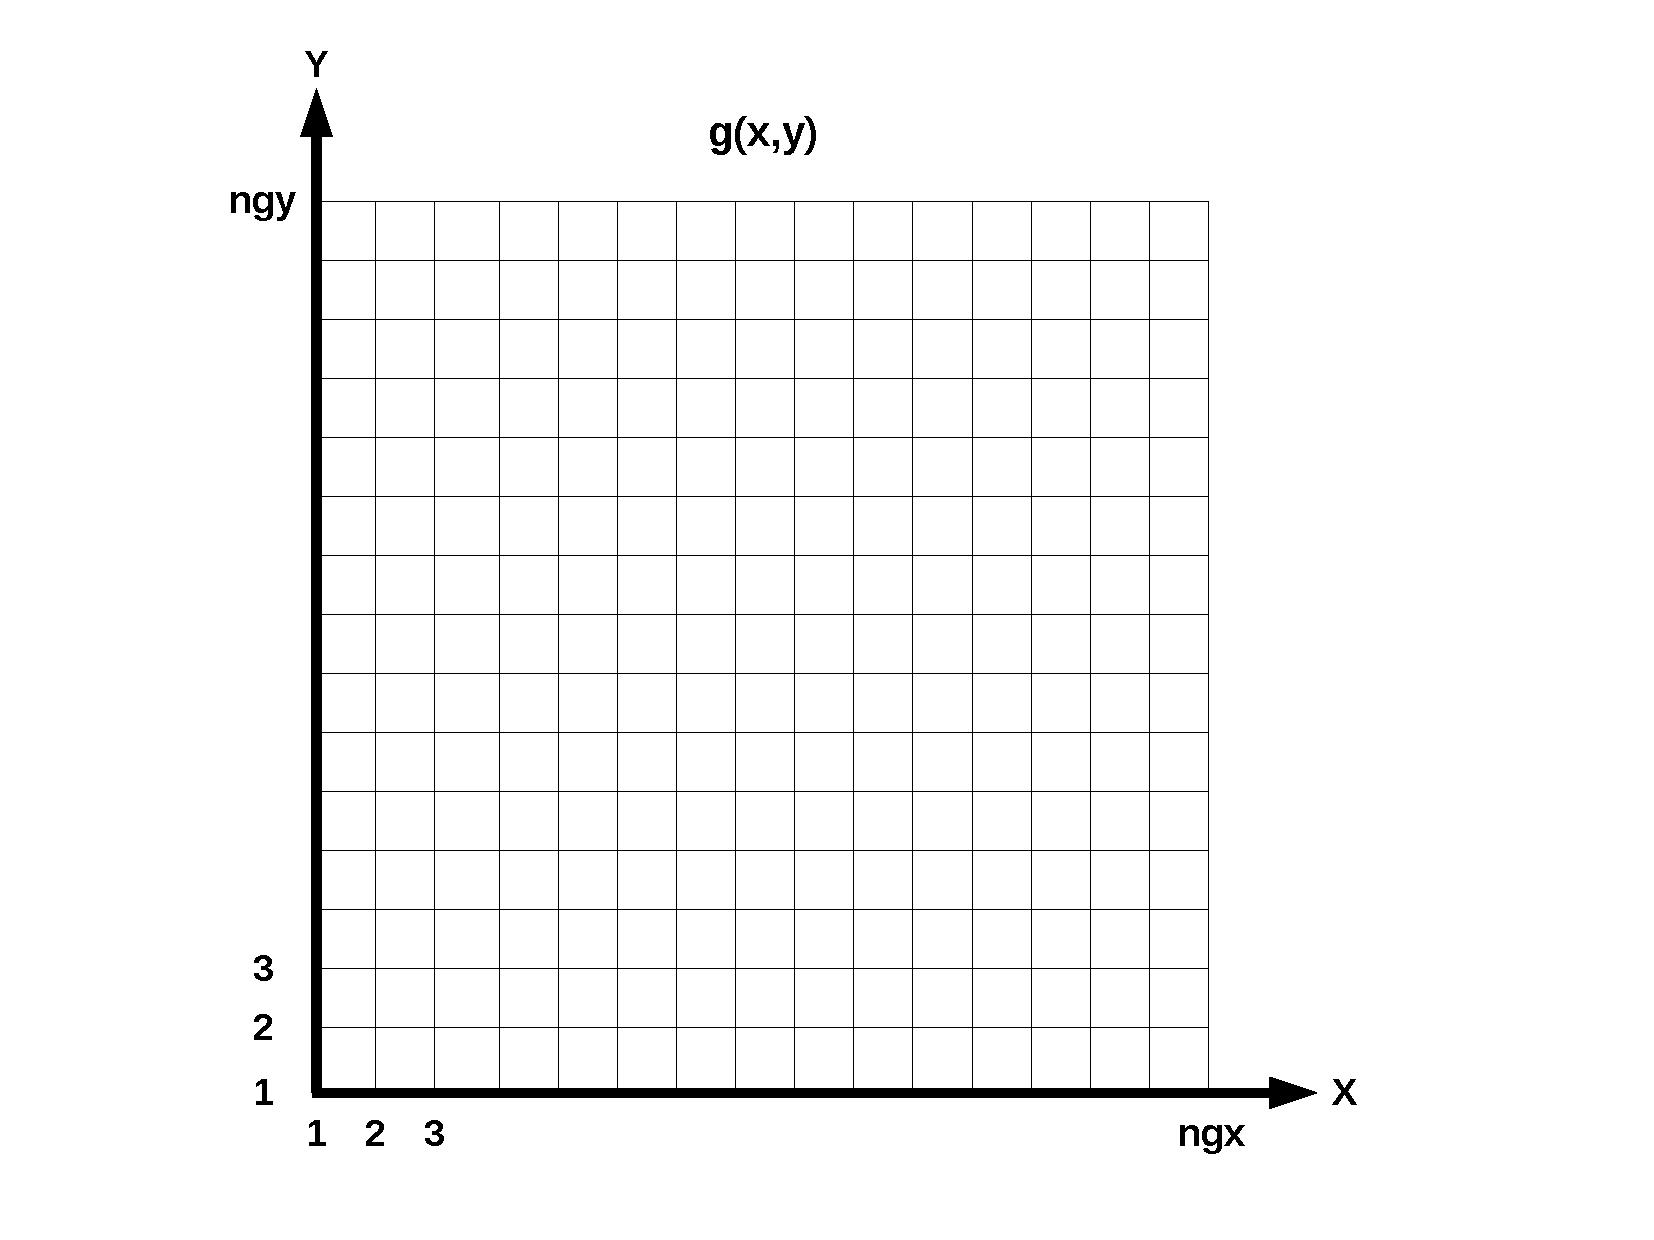
\includegraphics[height=9cm]{figures/phys_grid.pdf}
   \caption{In physical space functions $g(x,y)$ are represented on a
            regular grid with $ngx$ grid points in $x$-direction and
            $ngy$ grid points in $y$-direction. At present in CAT only
            the default $ngx = ngy$ is implemented.}
   \label{fig_physgrid}
\end{figure}
In physical space all fields $g(x,y)$ are real and are represented on 
a regular grid. Figure \ref{fig_physgrid} shows the grid for a horizontal
resolution of $ngx = ngy = 16$. Grid point fields read or written by CAT
are given in this format. The corresponding fields in spectral space are 
complex. Internally in CAT they are either represented as complex 
$c(k_{x},k_{y})$ or as real $f(k_{x},k_{y})$ fields.
\begin{figure}
   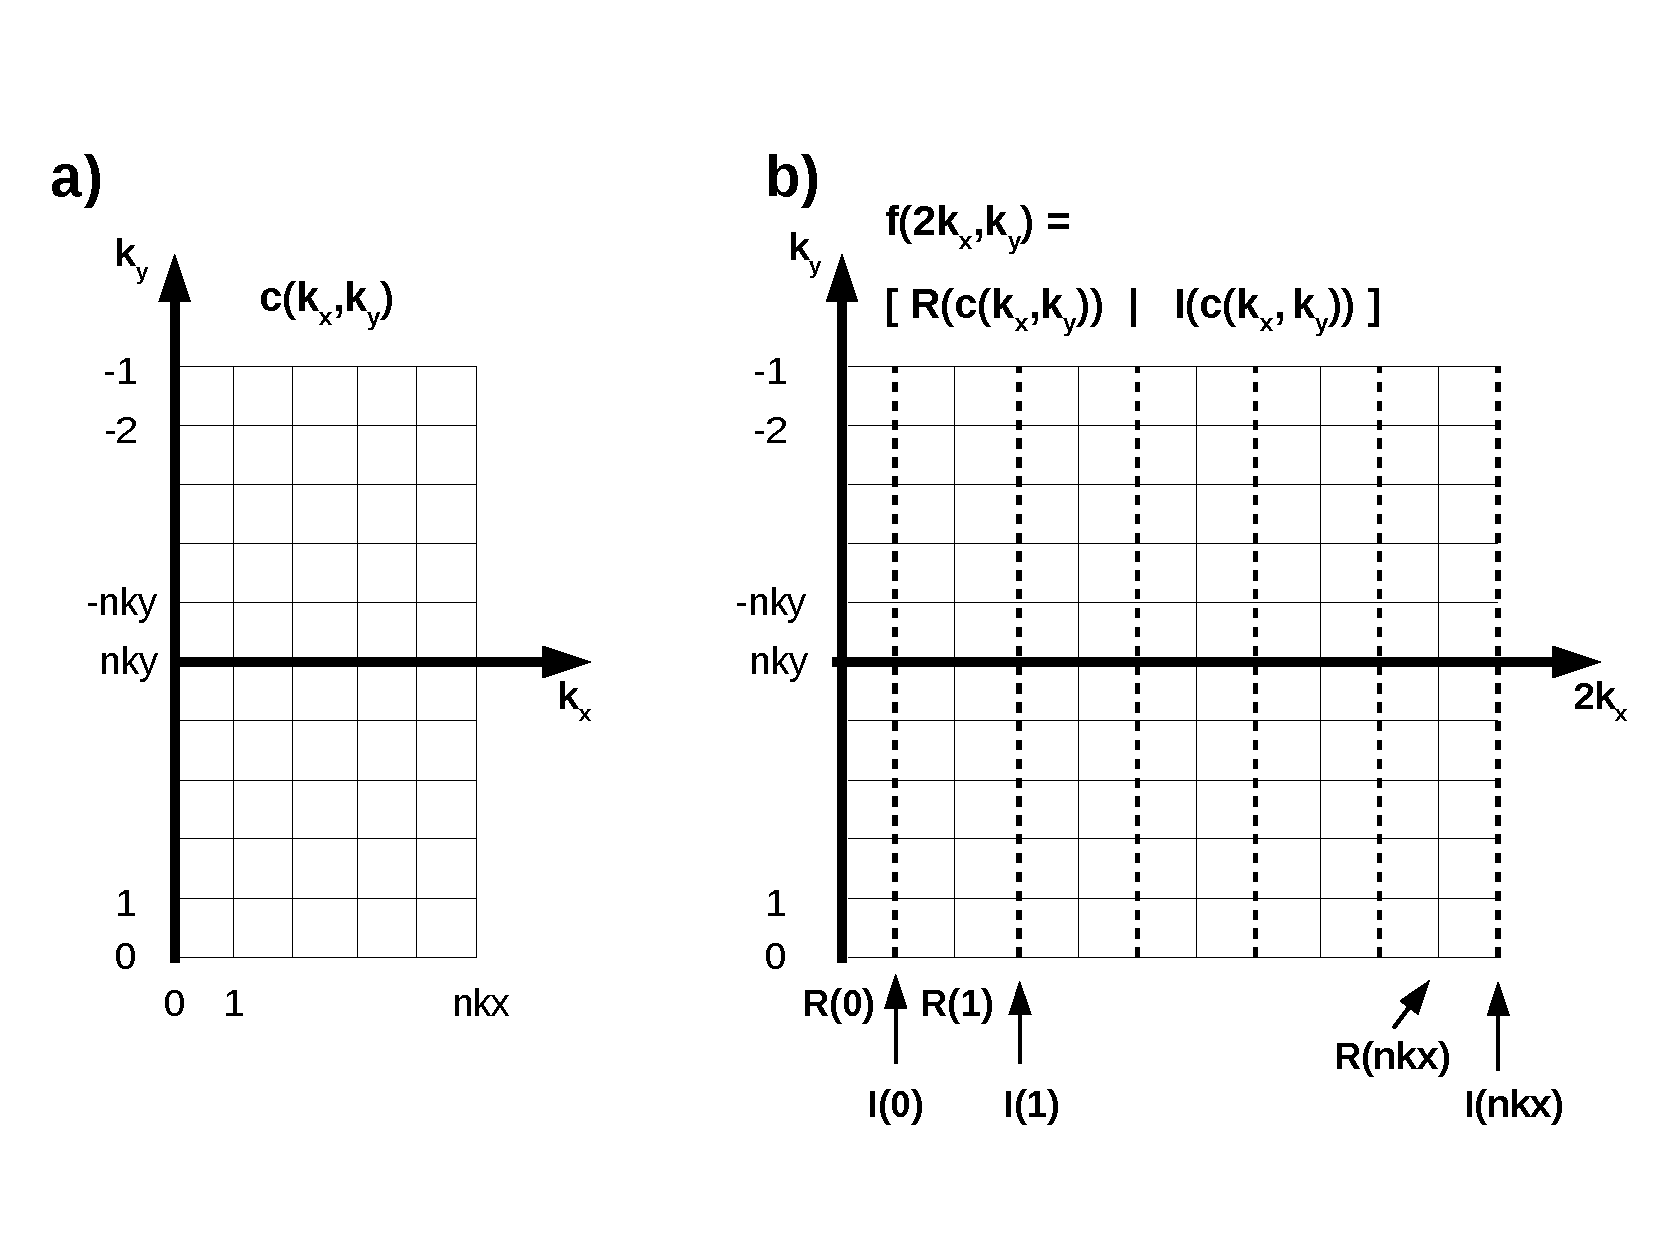
\includegraphics[height=11cm]{figures/cmplx_real_spec_grid.pdf}
   \caption{Functions in spectral space are represented either as
            complex fields $c$ (plate a) or as real fields $f$ containing
            in the first spectral coordinate $k_{x}$ the real and
            imaginary parts of $c$ in an alternating series (plate b).}
   \label{fig_ctorspecgrid}
\end{figure}
Plate (a) in figure \ref{fig_ctorspecgrid} shows the wave number
grid for the internal complex representation $c(k_{x},k_{y})$
of spectral fields. Due to the symmetry properties \ref{eq_symfourier}
it is sufficient to represent the spectral fields $c$ only on half of
the wave number space, i.e.\ only for the wave numbers
\begin{equation} \label{eq_ncentwgrid}
   (k_{x},\ k_{y}) \in  
   \{\ k_{x} \in [\ 0,1,\ \dots \ nkx \ ] \ \ \mbox{and} \ \ 
   k_{y} \in [\ 0, \ \dots \ ,nky,-nky, \ \dots \ , -1 \ ] \}.
\end{equation}
As described above we use the $2/3$-truncation, so that the bounds
$nkx$ and $nky$ are given by
\begin{equation} \label{eq_nkxnky}
   nkx = ngx/3 \ \ \mbox{and} \ \ nky = ngy/3,
\end{equation}
where the non-integer part of the division is omitted. In our example
$ngx=8$ from above $nkx = nky = 16$. The wave-numbers in $y$-direction
are not centered around zero. Plate (b) of figure \ref{fig_ctorspecgrid}
shows the internal real representation $f(k_{x},k_{y})$ of spectral fields.
In $y$-direction the spectral grid is the same for the complex $c$ and
the real representation $f$. In $x$-direction the number of coordinate
points is doubled for the real representation. Even coordinates starting
from $0$ hold the real part $\mathcal{R}(c(k_{x},k_{y}))$ and
the odd coordinates starting from 1 the imaginary part
$I(c(k_{x},k_{y}))$ of the complex fields $c(k_{x},k_{y})$.
This is on of the input/output formats of CAT. Prescribing complex spectral 
fields $c(k_{x},k_{y})$ in CAT it is important to keep in mind that on 
the $k_{y}$-axis ($k_{x} = 0$) values are not arbitrary, otherwise unphysical 
complex fields are created in grid point (physical) space. First $c(0,0)$ 
has to be real, they are the average of the field $g(x,y)$ in physical space. 
Taking the vorticity $cq$ we get for the special case of a doubly periodic 
domain $cq(0,0) = 0$. For the remaining values $(0,k_{y})$ the symmetry properties
\ref{eq_symfourier} have to be satisfied, i.e.\ on the $k_{y}$-axis
spectral fields must satisfy the condition $c(0,k_{y}) = c^{*}(0,-k_{y})$.
\begin{figure}
   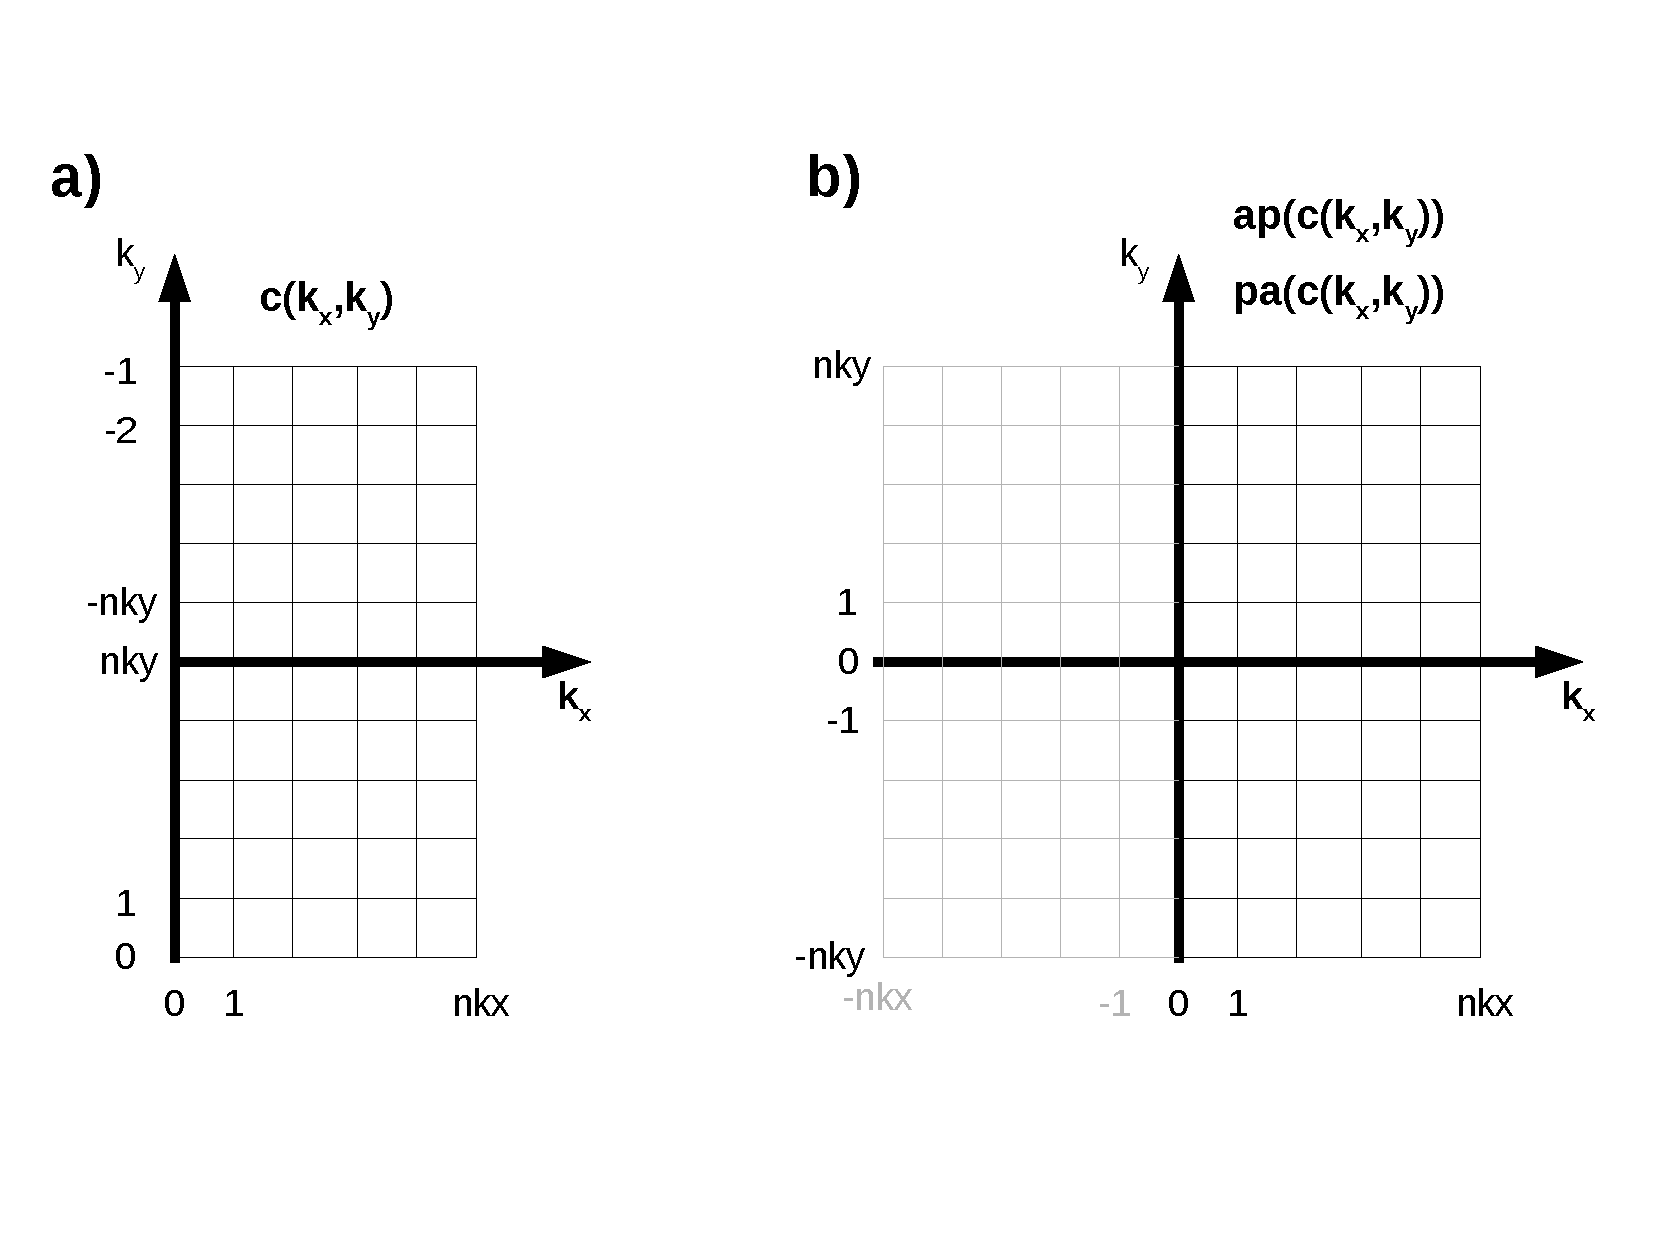
\includegraphics[height=11cm]{figures/cmplx_cent_grid.pdf}
   \caption{Internally (plate a) complex spectral fields $c$ are defined on
            the non-centered wave number grid given by (\ref{eq_ncentwgrid}).
            To visualize complex spectral fields and for i/o purposes (plate b) 
            amplitudes $ap(c)$ and phases $pa(c)$ are used (\ref{eq_centwgrid}).}
   \label{fig_cspecgrid}
\end{figure}
A second representation of complex fields for the Graphical User Interface 
(GUI) and for i/o purposes are the amplitudes $ap(c)$ and phases $pa(c)$  
defined on the positive part of the centered wave-number grid 
\begin{equation} \label{eq_centwgrid}
   (k_{x},\ k_{y}) \in  
   \{\ k_{x} \in [\ -nkx, \ \dots \ ,nkx \ ] 
    \ \ \mbox{and} \ \ 
       k_{y} \in [\ -nky, \ \dots \ ,nky \ ] \ \}.
\end{equation}
The amplitudes $ap(c)$ and phases $pa(c)$ of a complex field are determined
as follows
\begin{equation} \label{eq_c2amppha}
   ap(k_{x},k_{y}) = \sqrt{\mathcal{R}^{2}(c) + I^{2}(c)}
   \ \ \mbox{and} \ \ 
   pa(k_{x},k_{y}) = \tan^{-1}(\frac{I(c)}{\mathcal{R}(c)}).
\end{equation}
By the symmetry properties \ref{eq_symfourier} of spectral fields $c$
the amplitudes $ap(c)$ are symmetric with respect to the $k_{y}$-axis
and the phases $pa(c)$ are point symmetric with respect to the origin
$(0,0)$ of the grid of wave numbers. For visualization amplitudes $ap$
and phases $pa$ are represented on the left half space of centered
wave numbers denoted by the solid bold black grid given in plate (b)
of figure \ref{fig_cspecgrid} including the $k_{y}$-axis.

Using the amplitudes $ap(k_{x},k_{y})$ and phases $pa(k_{x},k_{y})$ 
defined on the positive $k_{x}$ part of the grid (\ref{eq_ncentwgrid}) 
one can represent a complex field $c(k_{x},k_{y})$ as follows
\begin{equation} \label{eq_amppha2c}
   c(k_{x},k_{y}) = ap(c(k_{x},k_{y})) \ 
       exp \left[ \ i \ pa(c(k_{x},k_{y})) \right].
\end{equation} 
%
\section{Evolution equations in Fourier space}
\label{sec_evolfourier}
%
The basic advantage of the Fourier representation is that
differential operators as $\partial_{x}$,
$\partial_{y}$, $\partial_{x} \partial_{y}$, $\nabla$, $\Delta$
are transformed to simple multiplication operators
$i k_{x}$, $i k_{y}/r$, $- k_{x} k_{y}/r$ ,$(i k_{x},i k_{y}/r)$, 
$-(k_{x}^{2} + k_{y}^{2}/r^{2})$ in spectral space with $i = \sqrt{-1}$.
Differential equations in physical space are thus reduced to algebraic 
equations in spectral space.

In the Fourier space it is now straight forward to determine
the stream function $\hat{\psi}(k_{x},k_{y},t)$ and the corresponding
velocity fields $\hat{u}(k_{x},k_{y},t)$ and $\hat{v}(k_{x},k_{y},t)$ once
the vorticity field $\hat{q}(k_{x},k_{y},t)$ is known. The
vorticity equation (\ref{eq_vortquasi2Dbaro}) of the quasi-2D
rotating case reduces to
\begin{equation} \label{eq_fourvortquasi2Dbaro}
 -\left(k_{x}^{2} + \frac{k_{y}^{2}}{r^{2}} + \alpha^{2} \right) 
  \hat{\psi}(k_{x},k_{y},t)
  =
 \hat{q}(k_{x},k_{y},t),
\end{equation}
which in the case for $\alpha \ne 0$ can always be solved for the
stream function
\begin{equation} \label{eq_psihatqhat}
  \hat{\psi}(k_{x},k_{y},t)
  =
  - \frac{1}
  {k_{x}^{2} + k_{y}^{2}/r^{2} + \alpha^{2}} \
  \hat{q}(k_{x},k_{y},t).
\end{equation}
In the case $\alpha = 0$ equation (\ref{eq_psihatqhat}) is still
valid except for the zero mode. Here we set $\hat{\psi}(0,0,t) = 0$,
which is consistent with the definition (\ref{eq_hquasi2Dbaropsi})
of the stream function and the double periodic boundary conditions.
Further the velocity field is simply given by
\begin{equation} \label{eq_uhat}
 \hat{u}(k_{x},k_{y},t) 
  =  -i \frac{k_{y}}{r} \ \hat{\psi}(k_{x},k_{y},t)
  = i \ \frac{k_{y}/r }
  {k_{x}^{2} + k_{y}^{2}/r^{2} + \alpha^{2}} \
  \hat{q}(k_{x},k_{y},t)
\end{equation}
and
\begin{equation} \label{eq_vhat}
 \hat{v}(k_{x},k_{y},t) = i k_{x} \ \hat{\psi}(k_{x},k_{y},t)
  = - i \ \frac{k_{x}}
  {k_{x}^{2} + k_{y}^{2}/r^{2} + \alpha^{2}} \
  \hat{q}(k_{x},k_{y},t).
\end{equation}

In spectral space the evolution equations of the general quasi-2D 
rotating case can be separated into individual ordinary differential 
equations. For every wave number pair $\mathbf{k} = (k_{x},k_{y})$ we get
\begin{equation}  \label{eq_evolqhat}
  \frac{d}{dt} \ \hat{q}_{\mathbf{k}}
   =
   i \ \frac{k_{x} \beta}{k_{x}^{2} + k_{y}^{2}/r^{2} + \alpha^{2}} 
     \ \hat{q}_{\mathbf{k}}
   -   \hat{J}_{\mathbf{k}}
   +   \hat{F}_{\mathbf{k}}
   +   \hat{D}_{\mathbf{k}}.
\end{equation}
For vanishing Jacobian, Forcing and Dissipation terms we get a linear 
equation
\begin{equation}  \label{eq_evolqhat_lin}
  \frac{d}{dt} \ \hat{q}_{\mathbf{k}}
   =
   i \ \frac{k_{x} \beta}{k_{x}^{2} + k_{y}^{2}/r^{2} + \alpha^{2}} 
     \ \hat{q}_{\mathbf{k}}
\end{equation}
which can be solved exactly 
\begin{equation} \label{eq_qhatbetasol}
 \hat{q}_{\mathbf{k}}(t)
  = 
 \exp
  \left[
   i \ \frac{k_{x} \beta}{k_{x}^{2} + k_{y}^{2}/r^{2} + \alpha^{2}} \
   \Delta t 
  \right] 
 \ \hat{q}_{\mathbf{k}}(t_{0}),
\end{equation}
with $\hat{q}_{\mathbf{k}}(t_{0})$ the initial condition at time $t_{0}$
and the time interval $\Delta t = t - t_{0}$. The $\beta$-term induces
a wave number dependend phase-shift. If one includes a linear
dissipation term $\hat{D}_{\mathbf{k}}$ the evolution equation can still 
be solved exactly (see section \ref{sec_dissipation}). The Jacobian 
$\hat{J}_{\mathbf{k}}$, forcing $\hat{F}_{\mathbf{k}}$ and dissipation 
$\hat{D}_{\mathbf{k}}$ terms are described in detail below.
%
\section{Jacobian} 
\label{sec_jacobian} 
%
The non-linearity of the Jacobian makes it numerically too expensive 
to solve it exclusively in spectral space. The individual terms in 
the products of the Jacobian are first differentiated in spectral
space and then transformed back to the physical space. There the terms 
are multiplied and the products are then transformed back to spectral 
space. Due to this back and forth transfomations the method is not  
purely spectral and is called pseudo-spectral method, see e.g.\ 
\cite{kreissandoliger1972} and \cite{orszag1972}. Due to the products 
the higher wave numbers have to be filtered out. In CAT trunction is 
used, see above. 

We present four different forms of the Jacobian $J$ in physical space, 
see equations (\ref{eq_2Dvortstream}), (\ref{eq_2Dflux}), 
(\ref{eq_2DJacobi2}) and (\ref{eq_2DJacobi4}). Using the pseudo-spectral 
method for each form we get a different representation of the 
Jacobian $\hat{J}$ in spectral space.   

For the Jacobian (\ref{eq_2Dvortstream}) of the first form
\begin{equation} \label{eq_jacobian01}
  J(\psi,\zeta) 
   = 
  J(\psi,q) 
   = 
  \psi_{x} \ q_{y} 
   -   
  q_{x} \  \psi_{y}
   =
   v \ q_{y}  + u \  q_{x},
\end{equation}
one proceeds as follows. First the individual differential terms 
are determined in spectral space using the fourier transform of 
vorticity, and the spectral representation of the differential 
operators. The basic operators are given by 
\begin{eqnarray} \label{eq_jacobian01_termsa}
  \mathcal{F}(\psi_{x})
  &=& 
  i  k_{x} \ \mathcal{F}(\psi)
   =
  \phantom{-} \mathcal{F}(v)
   = 
  - \ i \ \frac{k_{x}}{k^{2}_{x} + k^{2}_{y} + \alpha} \ 
  \mathcal{F}(q),
  \ \ 
  \mathcal{F}(q_{y})
   = 
  i k_{y} \ \mathcal{F}(q) \ \ \
  \\ \label{eq_jacobian01_termsb}
  \mathcal{F}(\psi_{y})
  &=&
  i  k_{y} \ \mathcal{F}(\psi)
   =
  - \mathcal{F}(u)
   = 
  - \ i \ \frac{k_{y}}{k^{2}_{x} + k^{2}_{y} + \alpha} \ 
  \mathcal{F}(q),
  \ \
  \mathcal{F}(q_{x})
   = 
  i k_{x} \ \mathcal{F}(q). \ \ \ 
\end{eqnarray}
Next all four terms defined by equations (\ref{eq_jacobian01_termsa}) 
and (\ref{eq_jacobian01_termsb}) are transformed to physical space. 
In physical space the Jacobian $J(\psi,\zeta)$ is then 
calculated following the definition (\ref{eq_jacobian01}) and finally
transformed back to spectral space. The Jacobian in spectral space 
$\hat{J}$ is given by
\begin{equation} \label{eq_jacobian01_J}
  \hat{J} 
   = 
  \mathcal{F}(v q_{y})
   +
  \mathcal{F}(u q_{x})
   = 
  \mathcal{F}(v q_{y} + u q_{x}).
\end{equation}
Combining all necessary steps we can write
\begin{equation} \label{eq_jacobian01_Jall}
  \hat{J} 
   =
  \mathcal{F}
   \left[
    \mathcal{F}^{-1} 
     \left(
       - i \frac{k_{x}}{k^{2}_{x}+k^{2}_{y}+\alpha} \ 
      \hat{q}
     \right) 
    \mathcal{F}^{-1} 
     \left(
      ik_{y} \ \hat{q}
     \right)
       +
    \mathcal{F}^{-1} 
     \left(
      i \frac{k_{y}}{k^{2}_{x}+k^{2}_{y}+\alpha} \ 
      \hat{q}
     \right) 
    \mathcal{F}^{-1}
     \left(
      ik_{x} \ \hat{q}
     \right)
   \right],
\end{equation}
where $\hat{q}$ is the vorticity in spectral space, the starting point
for a new time step. As can be seen one needs $5$ $2D$-FFT operations
to determine the Jacobian. The components of the Jacobian 
$\hat{J}_{k}$ are then used to determine the time 
evolution of the different wave number components of the vorticity 
$\hat{q}_{\mathbf{k}}$, see equation (\ref{eq_evolqhat}). 

In the flux form of the evolution equation ({\ref{eq_2Dflux}})
the second form of the Jacobian arises
\begin{equation} \label{eq_jacobian02}
  J(\psi,q) = (u \ q)_{x} + (v \ q)_{y}.
\end{equation}
Following again equations (\ref{eq_jacobian01_termsa}) and 
(\ref{eq_jacobian01_termsb}) we determine $\mathcal{F}(u)$ and
$\mathcal{F}(v)$. Then $\mathcal{F}(u)$, $\mathcal{F}(v)$ and 
$\mathcal{F}(q)$ are transformed to the physical
space,where the products $uq$ and $vq$ are formed. Finally the
products are transformed back to spectral space where they 
are differentiated. The Jacobian $\hat{J}$ in spectral space is
then given by
\begin{equation} \label{eq_jacobian02_J}
  \hat{J}
   = 
  i  k_{x} \ \mathcal{F}(uq)
   + 
  i  k_{y} \ \mathcal{F}(vq).
\end{equation}
Combining again all necessary steps we can write
\begin{eqnarray} \nonumber
  \hat{J} 
   &=&
  ik_{x} \ 
  \mathcal{F}
   \left(
    \mathcal{F}^{-1} 
     \left(
     \ i \frac{k_{y}}{k^{2}_{x}+k^{2}_{y}+\alpha} \ 
      \hat{q}
     \right) 
     \mathcal{F}^{-1}
      \left( \hat{q} \right)
   \right)
    \\ \label{eq_jacobian02_Jall}
   &+&
  ik_{y} \ 
  \mathcal{F}
   \left(
    \mathcal{F}^{-1} 
     \left(
      \ - \ i \frac{k_{x}}{k^{2}_{x}+k^{2}_{y}+\alpha} \ 
      \hat{q}
     \right) 
     \mathcal{F}^{-1}
      \left( \hat{q} \right)
   \right).
\end{eqnarray}
As we can see the Jacobian in spectral space $\hat{J}$ can now be 
determined by $5$ FFT operations.

The third form of the Jacobian in equation (\ref{eq_2DJacobi2})
is given by
\begin{equation} \label{eq_jacobian03}
  J(\psi,q) = (\psi \ q_{y})_{x} - (\psi \ q_{x})_{y}.
\end{equation}
In spectral space we get 
\begin{equation} \label{eq_jacobian03_J}
  \hat{J} = -ik_{x} \ \mathcal{F}(\psi \ q_{y}) 
            +ik_{y} \ \mathcal{F}(\psi \ q_{x}).
\end{equation}
Combining all necessary steps the Jacobian is determined by
\begin{eqnarray} 
  \hat{J} 
   &=& 
 -ik_{x} \ 
  \mathcal{F}\left(
     \mathcal{F}^{-1} 
       \left(-\frac{1}{k_{x}^{2} + k_{y}^{2} + \alpha} \ \hat{q} \right) \
     \mathcal{F}^{-1}
       \left(
         -ik_{y} \ \hat{q}
       \right)
             \right) 
    \\ \label{eq_jacobian03_Jall}
   &+&
  ik_{y} \ 
  \mathcal{F}\left(
     \mathcal{F}^{-1} 
       \left(-\frac{1}{k_{x}^{2} + k_{y}^{2} + \alpha} \ \hat{q} \right) \
     \mathcal{F}^{-1}
       \left(
         -ik_{x} \ \hat{q}
       \right)
             \right).
\end{eqnarray}
The fourth form of the Jacobian used in equation (\ref{eq_2DJacobi4}) is \begin{equation} \label{eq_jacobian04}
  J(\psi,q)
   = 
  \partial_{x}\partial_{y} \left(v^{2} - u^{2} \right)
   +
  \left( \partial^{2}_{x} - \partial^{2}_{y} \right)  uv.
\end{equation}
In this representation it is possible to reduce the number of FFT
operations from $5$ to $4$. We first have to determine $\hat{u}$ 
and $\hat{v}$ following equations (\ref{eq_jacobian01_termsa}) and 
(\ref{eq_jacobian01_termsa}) and then to transform them to physical 
space where the products $v^{2} - u^{2}$ and $uv$ are formed.
Finally we have to transform them back to spectral space where they
are differentiated. The Jacobian in spectral space $\hat{J}$ is 
given by   
\begin{equation} \label{eq_jacobian04_J}
  \hat{J}
   = 
  -k_{x}k_{y} \ \mathcal{F}(v^{2} - u^{2})
   +
   \left( k^{2}_{x} - k^{2}_{y} \right) \mathcal{F}(uv)
\end{equation} 
or by combining all necessary steps
\begin{eqnarray} \nonumber
  \hat{J} 
   &=&
  - \ k_{x}k_{y} \ 
  \mathcal{F}
   \left(
    \left[ 
     \mathcal{F}^{-1} 
     \left(
      \ - \ i \frac{k_{x}}{k^{2}_{x}+k^{2}_{y}+\alpha} \ 
      \hat{q}
     \right) 
    \right]^{2}
       -
    \left[ 
     \mathcal{F}^{-1} 
      \left(
      \ i \frac{k_{y}}{k^{2}_{x}+k^{2}_{y}+\alpha} \ 
       \hat{q}
      \right) 
    \right]^{2}
   \right)
    \\ \label{eq_jacobian02_Jall}
   &+&
  \left( k^{2}_{x} - k^{2}_{y} \right) \ 
  \mathcal{F}
   \left(
    \mathcal{F}^{-1} 
     \left(
     \ i \frac{k_{y}}{k^{2}_{x}+k^{2}_{y}+\alpha} \ 
      \hat{q}
     \right) 
    \mathcal{F}^{-1} 
     \left(
      \ - \ i \frac{k_{x}}{k^{2}_{x}+k^{2}_{y}+\alpha} \ 
      \hat{q}
     \right) 
   \right).
\end{eqnarray}
One can also use hybrid forms of the Jacobian which are a linear 
combination of the three forms given above.
%
\section{Dissipation} 
\label{sec_dissipation}
%
In CAT the default parameterization of viscosity (internal dissipation) 
and friction (dissipation at the horizontal boundaries of the fluid) 
is based on positive and negative powers of the Laplacian 
(see equation \ref{eq_Laplace_dissip}). In spectral space the dissipation
operator is given by the linear superposition
\begin{equation} \label{eq_Laplace_dissip_Fourier}
   \hat{D}_{\mathbf{k}}  \hat{q}_{\mathbf{k}}
    = - \left[
         \sigma \left(k_{x}^{2} + k_{y}^{2} \right)^{p_{\sigma}}
            + 
         \lambda \left(k_{x}^{2} + k_{y}^{2} \right)^{p_{\lambda}}
        \right]
        \hat{q}_{\mathbf{k}}.
\end{equation}
Using the definitions $\sigma$ and $\lambda$ of (\ref{eq_siglam})
we can write the dissipation operator (\ref{eq_Laplace_dissip_Fourier})
in the form
\begin{equation} \label{eq_Laplace_dissip_Fourier2}
   \hat{D}_{\mathbf{k}}  \hat{q}_{\mathbf{k}}
    = - \left[
         \frac{1}{t_{\sigma}} 
         \left(\frac{1}{k_{\sigma}}\right)^{2 p_{\sigma}}  
         \left(k_{x}^{2} + k_{y}^{2} \right)^{p_{\sigma}}
          + 
         \frac{1}{t_{\lambda}} 
         \left(\frac{1}{k_{\lambda}}\right)^{2 p_{\lambda}}
         \left(k_{x}^{2} + k_{y}^{2} \right)^{p_{\lambda}}
        \right]
        \hat{q}_{\mathbf{k}}.
\end{equation}
Mind that $p_{\lambda} \le 0$. A dissipation term based on
the superposition of powers of Laplacian is a multiplication
operator in the spectral space. Introducing the radius 
$r_{\mathbf{k}} = \sqrt{k^{2}_{x} + k^{2}_{y}}$ the dissipation 
operator can be written as  
\begin{equation} \label{eq_Laplace_dissip_Fourier3}
   \hat{D}_{\mathbf{k}}  \hat{q}_{\mathbf{k}}
    = 
   - \left[
       \sigma \ r^{2 p_{\sigma}}_{\mathbf{k}}
        +
       \lambda \ r^{2 p_{\lambda}}_{\mathbf{k}}
    \right]  
     \hat{q}_{\mathbf{k}}.
\end{equation}     
Using linear superpositions of different powers of the Laplacian as
defined in (\ref{eq_Laplace_dissip_poly}) we get in Fourier space
the more general dissipation operator
\begin{equation} \label{eq_Laplace_dissip_poly_Fourier}
  \hat{D}_{\mathbf{k}}  \hat{q}_{\mathbf{k}}
   =
  -
  \left[
   \sigma_{0} 
    +
   \sum_{n=1}^{n_{max}} 
    \left(
     \sigma_{n} \ r^{2n}_{\mathbf{k}}
      + 
     \lambda_{n} \ r^{-2n}_{\mathbf{k}}
    \right)
  \right] \ 
  \hat{q}_{\mathbf{k}},
\end{equation}
Including the dissipation operator described above into the
equation (\ref{eq_evolqhat_lin}) we get for every wave number $\mathbf{k}$ 
the linear evolution equation
\begin{equation}  \label{eq_evolqhat_linDiss}
  \frac{d}{dt} \ \hat{q}_{\mathbf{k}}
   =
  \left[
   i \ \frac{k_{x} \beta}{k_{x}^{2} + k_{y}^{2}/r^{2} + \alpha^{2}} 
    -
   \sigma_{0} 
    -
   \sum_{n=1}^{n_{max}} 
    \left[
     \sigma_{n} r^{2n}_{\mathbf{k}}
      + 
     \lambda_{n} r^{-2n}_{\mathbf{k}}
    \right]
  \right] \ \hat{q}_{\mathbf{k}},
\end{equation}
which has the exact solution
\begin{equation} \label{eq_Solevolqhat_linDiss}
 \hat{q}_{\mathbf{k}}(t_{0} + \Delta t)
  = 
 \exp
  \left[
    i \ \frac{k_{x} \beta}{k_{x}^{2} + k_{y}^{2}/r^{2} + \alpha^{2}}
   \ \Delta t 
  \right] 
  \ 
 \exp
  \left[
    - \sigma_{0}
    - \sum_{n=1}^{n_{max}} 
       \left(
        \sigma_{n} r^{2n}_{\mathbf{k}}
          + 
        \lambda_{n} r^{-2n}_{\mathbf{k}}
       \right)
   \Delta t 
  \right] 
 \ \hat{q}_{\mathbf{k}}(t_{0}),
\end{equation}
where $\hat{q}_{\mathbf{k}}(t_{0})$ is the initial condition at time $t_{0}$. 
As the solution (\ref{eq_Solevolqhat_linDiss}) shows the dissipation operator 
is a multiplication operator introducing a wave-number dependent exponential 
damping without phase shift.
Taking the form (\ref{eq_Laplace_dissip_Fourier2})
of the dissipation operator $\hat{D}_{\mathbf{k}}$ we can write the
time evolution corresponding to the dissipation operator 
(\ref{eq_Laplace_dissip_poly_Fourier}) as
\begin{equation} \label{eq_Solevolqhat_linDiss01}
 \hat{q}_{k}(t_{0} + \Delta t) 
  =    
 \exp
 -\left[
   \frac{\Delta t}{\tau_{\sigma,0}}  
    +
    \sum_{n=1}^{n_{max}} \ 
     \left( 
      \left(\frac{r_{\mathbf{k}}}{r_{\sigma,n}} \right)^{2n}
      \frac{\Delta t}{\tau_{\sigma,n}}
      \ - \ \left( \frac{r_{\mathbf{k}}}{r_{\lambda,n}} \right)^{-2n}
      \frac{\Delta t}{\tau_{\lambda,n}}
     \right) 
  \right] 
    \ \
 \hat{q}_{k}(t_{0}).
\end{equation}
Both representations (\ref{eq_Solevolqhat_linDiss}) and 
(\ref{eq_Solevolqhat_linDiss01}) are implemented in CAT. 
The first representation is the simplest way to implement dissipation. 
The second representation simplifies the set-up of a resolution independent
dissipation operator.   Starting with the parameters 
$r_{\sigma_{n}}$, $\tau_{\sigma_{n}}$, $r_{\lambda_{n}}$ and 
$\tau_{\lambda_{n}}$ for a given resolution, on has to keep
the damping time-scales for all resolutions and has to            


is most straightforward
representation 

we can

Using the representation (\ref{eq_Solevolqhat_linDiss}) we can
deduce the wave number radius dependent damping time scale (e-folding time)
$\tau_{\sigma_{n},k} = 1/()$

  deduce an intuitive picture 
for the damping properties of the different orders of the dissipation operator. 
The damping time scale (e-folding time) $\tau_{\sigma,0} = 1/\sigma_{0}$
of the $0$-order dissipation operator is independent of wave numbers. The 
other orders of the dissipation operator depend on the wave number scales 
$r_{\sigma},n$ and $r_{\lambda,n}$. We get the expressions
$\tau_{\sigma,n} = (1/r_{\sigma,n})^{2n} 1/\sigma_{n}$ and 
$\tau_{\lambda,n} = (r_{\lambda,n})^{2n} 1/\lambda_{n}$ which
after taking logarithms read 
\begin{equation}
  \log(\tau_{\sigma,n}) = -2n \ log(r_{\sigma,n}) - log(\sigma_{n})
  \ \ \mbox{and} \ \ 
  \log(\tau_{\lambda,n}) = 2n \ log(r_{\lambda,n}) - log(\lambda_{n}).
\end{equation}
As we see They depend on the radius of the 

In CAT the default dissipation operator for $nx = 64$, i.e.\ for $kx = 21$) 
is a superposition of small-scale friction ($n=2$) and hyperfriction 
of ($n=4$). The default reference wave numbers are 
$r_{\sigma,2} = r_{\sigma,4} = 21$ and the corresponding default 
damping time scales are $\tau_{\sigma,2} = $ and  $\tau_{\sigma,4} = $

  The parameter re chosen
in such a way that with the parameters     given by  


Considering the connection between convolutions and Fourier transforms   
$f * g = \hat{f} \hat{g}$ the dissipation operator can be seen as a 
special spectral filter. Using the filter approach one can introduce more
general spectral dissipation operators, which have no simple
correspondence in physical space. In general a filter in spectral space
cannot be expressed as a differential operator in physical space and so
introduces non-local effects there. A simple cut-off filter defined by
\begin{equation} \label{eq_cutoffDiss}
 \hat{q}_{\mathbf{k}}(t + \Delta t)
  = 
 \left\{
  \begin{array}{lcl}
   1 \ \hat{q}_{\mathbf{k}}(t)
    & 
   \mbox{for} \ \mathbf{k} \ \mbox{with}  
    & 
   r_{min} \leq |r_{\mathbf{k}}| \leq r_{max}
   \\
   0 \ \hat{q}_{\mathbf{k}}(t)
    &
   \mbox{otherwise}.
    &
  \end{array}
 \right.
\end{equation}
\begin{figure}
   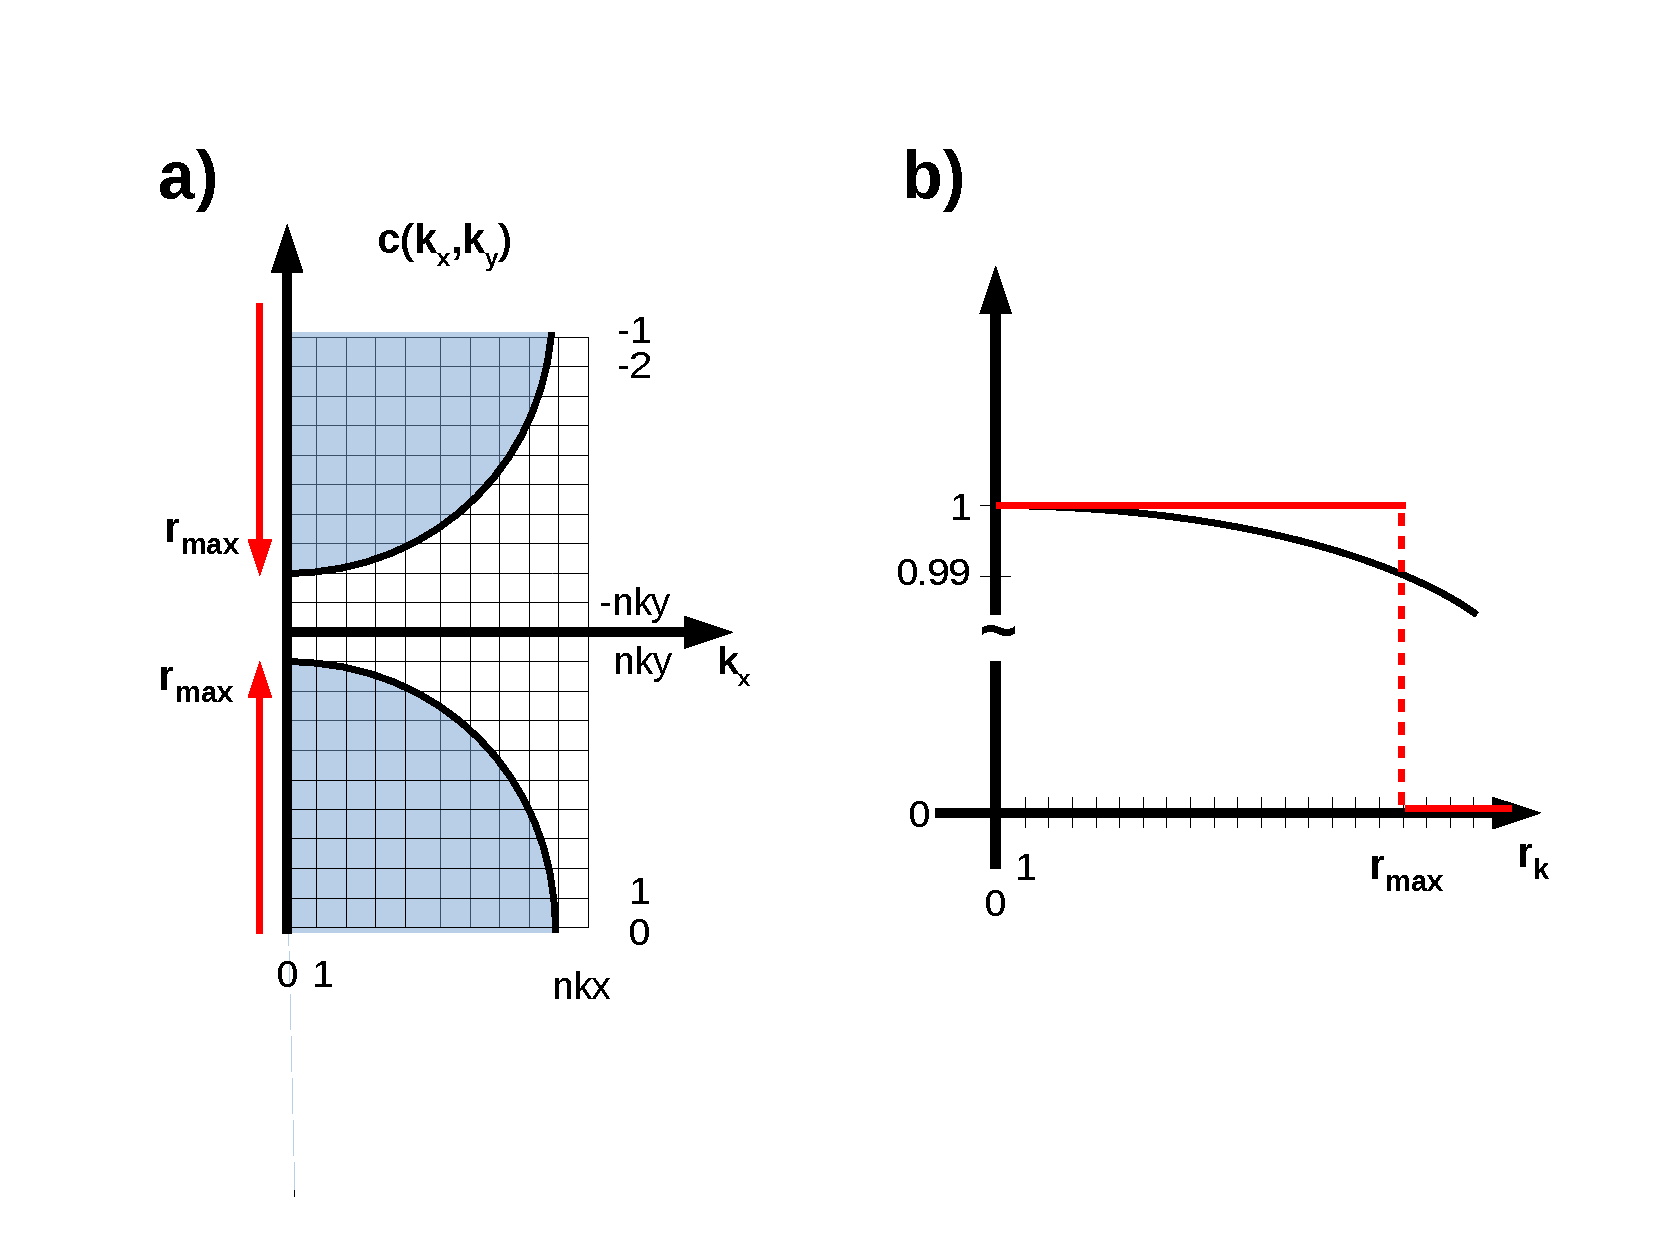
\includegraphics[height=10cm]{figures/diss_mask.pdf}
   \caption{Cut-off filter (plate a and red line in plate b)  and 
            the spectral representation of Laplacian friction (black line
            in plate b), i.e.\ the multiplication with a gaussian
            function.}
   \label{fig_diss_mask}
\end{figure}
is shown in figure \ref{fig_diss_mask}. Plate (a) shows how the
filter is defined as a zero/one mask. In Plate (b) the cut-off filter
(red line) is compared to the spectral representation of friction induced
by a Laplacian in physical space, which is the multiplication by a gaussian
function. One can generalize the cut-off filter by damping the small-scale
modes $r_{k} < r_{min}$ instead with zero by a factor 
$exp \left(- \Delta t/\tau_{damp} \right)$, where $\tau_{damp}$ is the
e-folding time of the small-scale modes. 
%
\section{Forcing and Pertubations}
\label{sec_forcing}
%
To specify a simulation with CAT completely one has to specify initial 
values, external forcings and perturbations where perturbations are
short external forcing pulses. For initial value problems the (potential)
vorticity field at the simulation start is needed. It can be prescribed 
as real grid point field in physical space or as complex field in spectral 
space. In CAT a complex field can be prescribed in two ways either as real 
and imaginary part or as amplitude and phase. For more details see the 
description of different field representations in section \ref{sec_grids}.

 the var0138 and can be specified . TIn physical space it can be specified as          



The forcing term $F$, see equation (\ref{eq_2Dvortvel}) in the non-rotating
case and equation in the rotating case (\ref{eq_quasi2Dbaro}), can be 
specified in either the physical or the spectral space. If a forcing is
prescribed in physical space it is transformed to spectral space before
it is applied to the dynamical equations. In addition to a constant forcing 
a time-dependent random forcing is implemented with a possible memory in time. 
In the mixed cases one can for example combine a constant large-scale forcing 
in physical space, e.g.\ a large-scale wind-stress, with a smale-scale random 
forcing, e.g.\ convective instability. A constant forcing in physical space
is prescribed by an input-file with variable code var1138, in can be given
in .  
%    
\section{Initialization}
\label{sec_initialization}
%

%
\section{Time-stepping schemes}
\label{sec_timestepping}
%
